\documentclass[reqno,a4paper,12pt]{amsart}

\usepackage{amsmath,amssymb,amsthm,geometry,xcolor,soul,graphicx}
\usepackage{titlesec}
\usepackage{enumerate}
\usepackage{lipsum}
\usepackage{listings}
\RequirePackage[most]{tcolorbox}
\usepackage{braket}
\usepackage{esint} %$\varoiint$ (带圈的二重积分)
\usepackage[colorlinks,linkcolor=red]{hyperref} %\url{}超链接
\usepackage{xeCJK}
\setCJKmainfont{Kai}
\geometry{left=0.7in, right=0.7in, top=1in, bottom=1in}

\renewcommand{\baselinestretch}{1.3}

\title{固体物理第四次作业}
\author{董建宇 ~~ 2019511017}

\begin{document}

\maketitle
\titleformat{\section}[hang]{\small}{\thesection}{0.8em}{}{}
\titleformat{\subsection}[hang]{\small}{\thesubsection}{0.8em}{}{}

\section{\textbf{(5.2) Effective Nuclear Charge and Ionization Energy}}
\begin{enumerate}[(a)]
	\item Let us approximate an electron in the $n^{th}$ shell (i.e., principal quantum number $n$) of an atom as being like an electron in the $n^{th}$ shell of a hydrogen atom with an effective nuclear charge $Z$. Use your knowledge of the hydrogen atom to calculate the ionization energy of this electron (i.e., the energy required to pull the electron away from the atom) as a function of $Z$ and $n$.
	\begin{tcolorbox}[breakable, colback = black!5!white, colframe = black]
	由波尔氢原子模型可知,轨道角动量量子化:
	\[
		mvr = n\hbar.
	\]
	库伦引力提供电子运动向心力得:
	\[
		\frac{1}{4\pi\epsilon_0}\frac{Ze^2}{r^2} = m\frac{v^2}{r}.
	\]
	可以解得电子能量为:
	\[
		E = \frac{1}{2}mv^2 - \frac{1}{4\pi\epsilon_0}\frac{Ze^2}{r} = -\frac{1}{2}mv^2 = -\frac{Z^2}{n^2} \frac{me^4}{2(4\pi\epsilon_0)^2\hbar^2} = -\frac{Z^2}{n^2}\times Ry.
	\]
	其中$Ry = 13.6eV$为里德伯常数。
	\end{tcolorbox}
	
	\item Consider the two approximations discussed in the text for estimating the effective nuclear charge: 
	\begin{itemize}
		\item (Approximation a) 
		\[
			Z = Z_{nuc} - N_{inside}
		\]
		\item (Approximation b)
		\[
			Z = Z_{nuc} - N_{inside} - (N_{same}-1)/2
		\]
	\end{itemize}
	where $Z_{nuc}$ is the actual nuclear charge (or atomic number), $N_{inside}$ is the number of electrons in shells inside of $n$ (i.e., electrons with principal quantum numbers $n'<n$), and $N_{same}$ is the total number of electrons in the $n^{th}$ principal shell (including the electron we are trying to remove from the atom, hence the -1). \\
	$\triangleright$ Explain the reasoning behind these two approximations. 
	\begin{tcolorbox}[breakable, colback = black!5!white, colframe = black]
	近似(a)是因为处于内层的电子可以近似中和原子核中的一个带电子电量正电荷对外层电子的影响,而处于更高能级的电子近似对内层电子没有影响。因此处于$n$能级的电子对应的有效核电荷数近似为:
	\[
		Z = Z_{nuc} - N_{inside}.
	\]
	近似(b)是在近似(a)的基础上考虑了同一层电子的影响。处于同一能级的电子,近似处于同一半径的轨道上,因此每一个电子近似拿出一半的电荷互相屏蔽,因而处于$n$能级的电子对应的有效核电荷数近似为:
	\[
		Z = Z_{nuc} - N_{inside} - (N_{same} - 1)/2.
	\]
	\end{tcolorbox}
	$\triangleright$ Use these approximations to calculate the ionization energies for the atoms with atomic number 1 through 21. Make a plot of your results and compare them to the actual ionization energies (you will have to look these up on a table). \\
	Your results should be qualitatively quite good. If you try this for higher atomic numbers, the simple approximations begin to break down. Why is this?
	\begin{tcolorbox}[breakable, colback = black!5!white, colframe = black]
	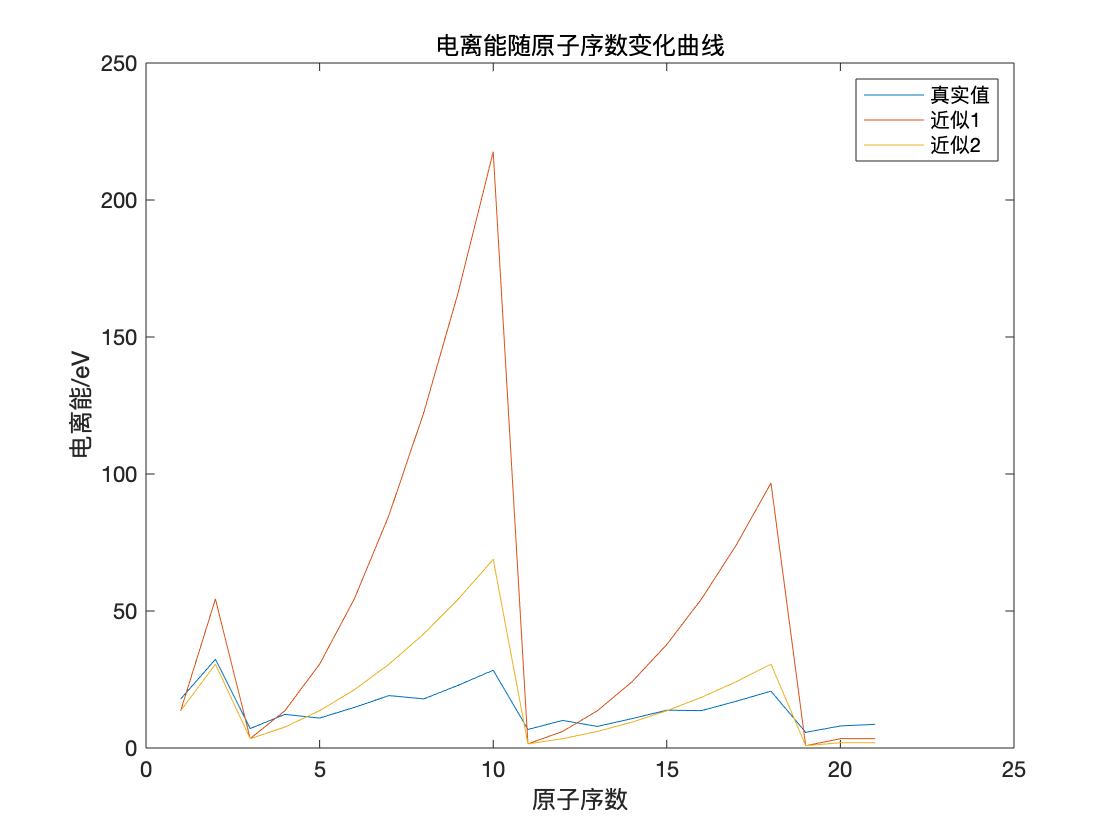
\includegraphics[scale = 0.35]{ionization.png}\\
	真实值数据源:\url{https://wenku.baidu.com/view/a210be663369a45177232f60ddccda38376be1cc.html} \\
	可以观察到:两种近似在趋势上与实际图线相似。但是数值上相差较大。在主量子数大于等于2的能级上,有不同能量的角量子数,因此如果将近似2优化为进一步区分角量子数的能量差,则可能在数值上更接近真实值。随着原子序数的增大,同一能级对应的角量子数也增多,同一能级的不同电子能量差也可能更大,因而近似条件被打破。与此同时,电子并不一定按照主量子数从低向高排列,比如$3d$轨道一般处在$4s$轨道的外层,因而电离并不一定是主量子数最大的能级上的电子。 \\
	综上,对于原子序数较大的原子,这两种简单的近似失效。
	\end{tcolorbox}
	
\end{enumerate}

\section{\textbf{(5.3) Exceptions to Madelung's Rule}}
\begin{enumerate}[(a)]
	\item Although Madelung's rule for the filling of electronic shells holds extremely well, there are a number of exceptions to the rule. Here are a few of them: 
	\begin{align*}
		Cu &= [Ar]4s^13d^{10} \\
		Pd &= [Kr]5s^04d^{10} \\
		Ag &= [Kr]5s^14d^{10} \\
		Au &= [Xe]6s^14f^{14}5d^{10}
	\end{align*}
	$\triangleright$ What should the electron configurations be if these elements followed Madelung's rule and the Aufbau principle? \\
	\begin{tcolorbox}[breakable, colback = black!5!white, colframe = black]
	如果这些元素遵循Madelung's rule和Aufbau principle,则电子分布应该为:
	\begin{align*}
		Cu &= [Ar]4s^23d^{9} \\
		Pd &= [Kr]5s^24d^{8} \\
		Ag &= [Kr]5s^24d^{9} \\
		Au &= [Xe]6s^24f^{14}5d^{9}
	\end{align*}
	\end{tcolorbox}
	$\triangleright$ Explain how the statement "3d is inside of 4s" might help justify this exception in copper.
	\begin{tcolorbox}[breakable, colback = black!5!white, colframe = black]
	对于铜而言,如果3d在4s内层,则3d能级能量低于4s能级的电子能量,为了使原子能量最低,则4d层电子会优先填满后再去填充3d能级。
	\end{tcolorbox}
\end{enumerate}

\section{\textbf{(6.2) Covalent Bonding in Detail*}}
\begin{enumerate}[(a)]
	\item Linear Combination of Atomic Orbitals: \\
	In section 6.2.2 we considered two atoms each with a single atomic orbital. We called the orbital $\ket{1}$ around nucleus 1 and $\ket{2}$ around nucleus 2. More generally we may consider any set of wavefunctions $\ket{n}$ for $n = 1,\cdots, N$. For simplicity, let us assume this basis is orthonormal $\langle n \vert m \rangle = \delta_{nm}$ \\
	Let us write a trial wavefunction for our ground state as 
	\[
		\ket{\Psi} = \sum_n \phi_n\ket{n}.
	\]
	This is known as a linear combination of atomic orbitals, LCAO, or tight binding (is is used heavily in numerical simulation of molecules). \\
	We would like to find the lowest-energ wavefunction we can construct in this form, i.e., the best approximation to the actual ground-state wavefunction. (The more states we use in our basis, generally, the more accurate our results will be.) We claim that the ground state us given by the solution of the effective Schroedinger equation 
	\[
		\mathcal{H} \phi = E\phi
	\]
	where $\phi$ is the vector of $N$ coefficients $\phi_n$, and $\mathcal{H}$ is the $N$ by $N$ matrix
	\[
		\mathcal{H}_{n,m} = \bra{n}H\ket{m}
	\]
	with $H$ the Hamiltonian of the full system we are considering, To prove this, let us construct the energy 
	\[
		E = \frac{\bra{\psi} H \ket{\psi}}{\langle \psi \vert \psi \rangle}
	\]
	$\triangleright$ Show that minimizing this energy with respect to each $\phi_n$ gives the same eigenvalue equation, Eq. 6.13. Similarly, the second eigenvalues of the effective Schrodinger equation will be an approximation to the first excited state of the system.
	\begin{tcolorbox}[breakable, colback = black!5!white, colframe = black]
	将$\ket{\psi}$在基矢上展开可得:
	\[
		\ket{\psi} = \sum_n \phi_n \ket{n}.
	\]
	则能量为:
	\[
		E = \frac{\bra{\psi} H \ket{\psi}}{\langle \psi \vert \psi \rangle} = \frac{\sum_{n,m} \phi_m^*\phi_n \bra{m} H \ket{n}}{\sum_n \vert \phi_n \vert^2} = \frac{\sum_{n,m} \phi_m^*\phi_n H_{m,n}}{\sum_n \vert \phi_n \vert^2}
	\]
	求偏微分可得:
	\[
		0 = \frac{\partial E}{\partial \phi_n} = \frac{\sum_m \phi_m^*H_{m,n}}{\sum_n \vert \phi_n \vert^2} - \frac{\sum_{n,m} \phi_m^*\phi_nH_{m,n}}{\sum_n \vert \phi_n \vert^2} \frac{\phi_n^*}{\sum_n \vert \phi_n \vert^2}.
	\]
	若态矢量满足归一化条件,则有:
	\[
		\sum_m \phi_m^* H_{m,n} - E\phi_n^* = 0.
	\]
	两侧取共轭可得:
	\[
		\sum_m \phi_m H_{n,m} = E \phi_n.
	\]
	则最小化能量将得到对应$\phi_n$的本征值方程。
	\end{tcolorbox}
	
	\item Two-orbital covalent bond \\
	Let us return to the case where there are only two orbitals in our basis. This pertains to a case where we have two identical nuclei and a single electron which will be shared between them to form a covalent bond. We write the full Hamiltonian as 
	\[
		H = \frac{\mathbf{p}^2}{2m} + V(\mathbf{r} - \mathbf{R_1}) + V(\mathbf{r} - \mathbf{R_2}) = K + V_1 + V_2
	\]
	where $V$ is the Coulomb interaction between the electron and the nucleus, $R_1$ is the position of the first nucleus and $R_2$ is the position of the second nucleus. Let $\epsilon$ be the energy of the atomic orbital around one nucleus in the absence of the other. In other word 
	\begin{align*}
		(K+V_1) \ket{1} &= \epsilon \ket{1} \\
		(K+V_2) \ket{2} &= \epsilon \ket{2}
	\end{align*}
	Define also the cross-energy element 
	\[
		V_{cross} = \bra{1} V_2 \ket{1} = \bra{2} V_1 \ket{2}
	\]
	and the hopping matrix element 
	\[
		t = -\bra{1} V_2 \ket{2} = - \bra{1} V_1 \ket{2}
	\]
	These are not typos! \\
	$\triangleright$ Why can we write $V_{cross}$ and $t$ equivalently using either one of the expressions given on the righthand side? \\
	$\triangleright$ Show that the eigenvalues of our Schroedinger equation Eq.6.1. are given by 
	\[
		E = \epsilon +V_{cross} \pm \vert t \vert
	\]
	$\triangleright$ Argue (perhaps using Gauss's law) that $V_{cross}$ should roughly cancel the repulsion between nuclei, so that, in the lower eigenstate total energy is indeed lower when the atoms are closer together. \\
	$\triangleright$ This approximation must fail when the atoms get sufficiently close. Why?
	\begin{tcolorbox}[breakable, colback = black!5!white, colframe = black]
	交叉能量部分表示$\mathbf{R_2}$处原子核与轨道1上的电子相互作用能量,由对称性可知,该能量等于$\mathbf{R_1}$处原子核与轨道2上的电子相互作用能量。因此$V_{cross}$可以用右式任意一个等价描述。 \\
	在计算Hamiltonian算符矩阵对应矩阵元$\bra{1} H \ket{2}$时,有:
	\[
		\bra{1} H \ket{2} = \bra{1} K + V_1 + V_2 \ket{2} = \epsilon_0 \langle 1 \vert 2 \rangle + \bra{1} V_2 \ket{2} = \bra{1} V_1 \ket{2} + \epsilon_0 \langle 1 \vert 2 \rangle
	\]
	则有:
	\[
		-\bra{1} V_2 \ket{2} = -\bra{1} V_1 \ket{2} = t.
	\]
%	对于$t$,由于Hamiltonian算符为厄米算符,则有:
%	\[
%		H_{12} = \bra{1} H \ket{2} = H_{21}^* = \bra{2} H \ket{1}^*.
%	\]
%	将Hamiltonian算符写成三个算符的和,则有:
%	\[
%		H_{12} = \bra{1} H \ket{2} = \bra{1} K + V_1 + V_2 \ket{2} = \epsilon_0 \langle 1 \vert 2 \rangle + \bra{1} V_1 \ket{2} = \bra{1} V_1 \ket{2}.
%	\]
%	\[
%		H_{21} = \bra{2} H \ket{1} = \bra{2} K + V_1 + V_2 \ket{1} = \epsilon_0 \langle 2 \vert 1 \rangle + \bra{2} V_1 \ket{1} = \bra{2} V_1 \ket{1}.
%	\]
%	即
%	\[
%		
%	\]
	薛定谔方程本征值方程为:
	\[
	\left\vert\begin{matrix}
		\epsilon + V_{cross} - E & -t \\
		-t^* & \epsilon + V_{cross} - E
	\end{matrix}\right\vert = (\epsilon + V_{cross} - E)^2 - \vert t \vert^2 = 0.
	\]
	可以解得:
	\[
		E = \epsilon + V_{cross} \pm \vert t \vert.
	\]
	交叉势能项为原子2上的电子感受到原子1的原子核吸引产生的势能。近似可以假设电子在原子核2附近球对称分布,由高斯定理可知:
	\[
		\frac{\sum q}{\epsilon_0} = \varoiint \vec{E} \cdot \,d\vec{S}
	\]
	则当两原子距离较大时(原子1的原子核在积分曲面的外侧),原子2上的电子屏蔽了原子2的原子核对原子1的原子核的影响。反之亦然。也就意味着在的能量本征态时(原子1的原子核在积分曲面的外侧),当原子靠近时,总能量变低。 \\
	但当两原子充分近时(原子1的原子核在积分曲面的外侧),电子并不能屏蔽两原子核的相互作用,同时,原子2上的电子与原子1的原子核的势能不再随着距离缩短而持续降低。除此之外,当两原子核充分近时,$\ket{1}$与$\ket{2}$的正交关系也不再近似满足。该近似必定失败。
	\end{tcolorbox}
\end{enumerate}

\section{\textbf{(6.3) LCAO and the Ionic-Covalent Crossover}}
\begin{enumerate}[(a)]
	\item For Exercise 6.2.b consider now the case where the atomic orbitals $\ket{1}$ and $\ket{2}$ have unequal energies $\epsilon_{0,1}$ and $\epsilon_{0,2}$. As the difference in these two energies increases show that the bonding orbital becomes more localized on the lower-energy atom. For simplicity you may use the orthogonality assumption $\langle 1 \vert 2 \rangle = 0$. Explain how this calculation can be used to describe a crossover between covalent and ionic bonding. 
	\begin{tcolorbox}[breakable, colback = black!5!white, colframe = black]
	不妨假设有:
	\[
		\epsilon_{0,1} < \epsilon_{0,2}.
	\]
	则Hamiltonian矩阵为:
	\begin{align*}
		H_{1,1} &= \bra{1} K + V_1 + V_2 \ket{1} = \epsilon_{0,1} + \bra{1} V_2 \ket{1}, \\
		H_{1,2} &= \bra{1} K + V_1 + V_2 \ket{2} = \bra{1} V_2 \ket{2} = -t, \\
		H_{2,1} &= \bra{2} K + V_1 + V_2 \ket{1} = -t^*, \\
		H_{2,2} &= \bra{2} K + V_1 + V_2 \ket{2} = \epsilon_{0,2} + \bra{2} V_1 \ket{2}.
	\end{align*}
	令$V_{cross} = \bra{1} V_2 \ket{1} = \bra{2} V_1 \ket{2}$,则本征值满足:
	\[
		\left\vert \begin{matrix}
			\epsilon_{0,1} + V_{cross} - E & -t \\
			-t^* & \epsilon_{0,2} + V_{cross} - E
		\end{matrix}\right\vert = 0
	\]
	可以解得:
	\[
		E = \frac{(\epsilon_{0,1}+\epsilon_{0,2}+2V_{cross}) \pm \sqrt{(\epsilon_{0,1} - \epsilon_{0,2})^2 + 4\vert t \vert^2}}{2}
	\]
	对于基态能量$E_{ground} = \frac{(\epsilon_{0,1}+\epsilon_{0,2}+2V_{cross}) - \sqrt{(\epsilon_{0,1} - \epsilon_{0,2})^2 + 4\vert t \vert^2}}{2}$,本征态矢量满足:
	\[
		\begin{pmatrix}
			\epsilon_{0,1} + V_{cross} & -t \\
			-t^* & \epsilon_{0,2} + V_{cross}
		\end{pmatrix}
		\begin{pmatrix}
			a \\
			b
		\end{pmatrix}
		= E_{ground}\begin{pmatrix}
			a \\
			b
		\end{pmatrix}
	\]
	则有:
	\[
		\frac{a}{b} = \frac{\sqrt{(\epsilon_{0,1} - \epsilon_{0,2})^2+4\vert t \vert^2} - (\epsilon_{0,1} - \epsilon_{0,2})}{t^*}, 
	\]
	\[
		\frac{b}{a} = \frac{\sqrt{(\epsilon_{0,1} - \epsilon_{0,2})^2+4\vert t \vert^2} + (\epsilon_{0,1} - \epsilon_{0,2})}{t}, 
	\]
	则可以计算得:
	\[
		\left\vert \frac{a}{b} \right\vert^2 - \left\vert \frac{b}{a} \right\vert^2 = -\frac{(\epsilon_{0,1} - \epsilon_{0,2})\sqrt{(\epsilon_{0,1} - \epsilon_{0,2})^2 + 4\vert t \vert^2}}{\vert t \vert^2}.
	\]
	则当$\epsilon_{0,1}<\epsilon_{0,2}$时,有:
	\[
		\left\vert \frac{a}{b} \right\vert^2 - \left\vert \frac{b}{a} \right\vert^2 > 0.
	\]
	即$\vert a \vert^2 > \vert b \vert^2$,也就意味着处于$\ket{1}$态的概率高。反之,当$\epsilon_{0,1}>\epsilon_{0,2}$时,同理可得,处于$\ket{2}$态的概率高。\\
	综上所述,成键轨道更多的概率处在低能量的原子。
	\end{tcolorbox}
\end{enumerate}

\section{\textbf{(6.4) Ionic Bond Energy Budget}}
\begin{enumerate}[(a)]
	\item The ionization energy of a sodium atom is about $5.14eV$. The electron affinity of a chlorine atom is about $3.62 eV$. When a singlesodium atom bonds with a single chlorine atom, the bond length is roughly $0.236nm$. Assuming that the cohesive energy is purely Coulomb energy, calculate the total energy released when a sodium atom and a chlorine atom come together to form a NaCl molecule. Compare your result to the experimental value of $4.26eV$. Qualitatively account for the sign of your error.
	\begin{tcolorbox}[breakable, colback = black!5!white, colframe = black]
	假设结合能只有库伦势能,则结合能为:
	\[
		E_{bond} = \frac{e^2}{4\pi\epsilon_0d} \approx 6.10 eV.
	\]
	则释放的总能量为:
	\[
		E_{total} = -E_{Na} + E_{Cl} + E_{bond} = -5.14eV + 3.62eV + 6.10eV = 4.58eV.
	\]
	比实验值$4.26eV$高。原因可能是在原子靠近形成离子键时,存在一个短程排斥力,会降低释放的总能量,因此实验测量到的能量低于“只存在库伦势能”假设下的计算值。
	\end{tcolorbox}
\end{enumerate}


\end{document}